%%%INTRODUCCIÓN GENERAL%%%
\chapter*{Introducción}
\addcontentsline{toc}{chapter}{Introducción}


El prefijo nano deriva del griego \emph{nanos}, que significa literalmente ``enano''. En el sistema internacional de unidades, el prefijo nano representa un factor de $\mathrm{10^{-9}}$, o una mil millonésima. Al añadir el prefijo a la unidad de longitud, obtenemos ``nanómetro'' (nm), o una mil millonésima parte de un metro. Así la nanotecnología se define como la ciencia, tecnología, e ingeniería que trata sistemas en el rango aproximado de 1-100 nanómetros \citep{Haick2013,Gressler2013}.

\begin{figure}[h!]
	\centering
	\fbox{
		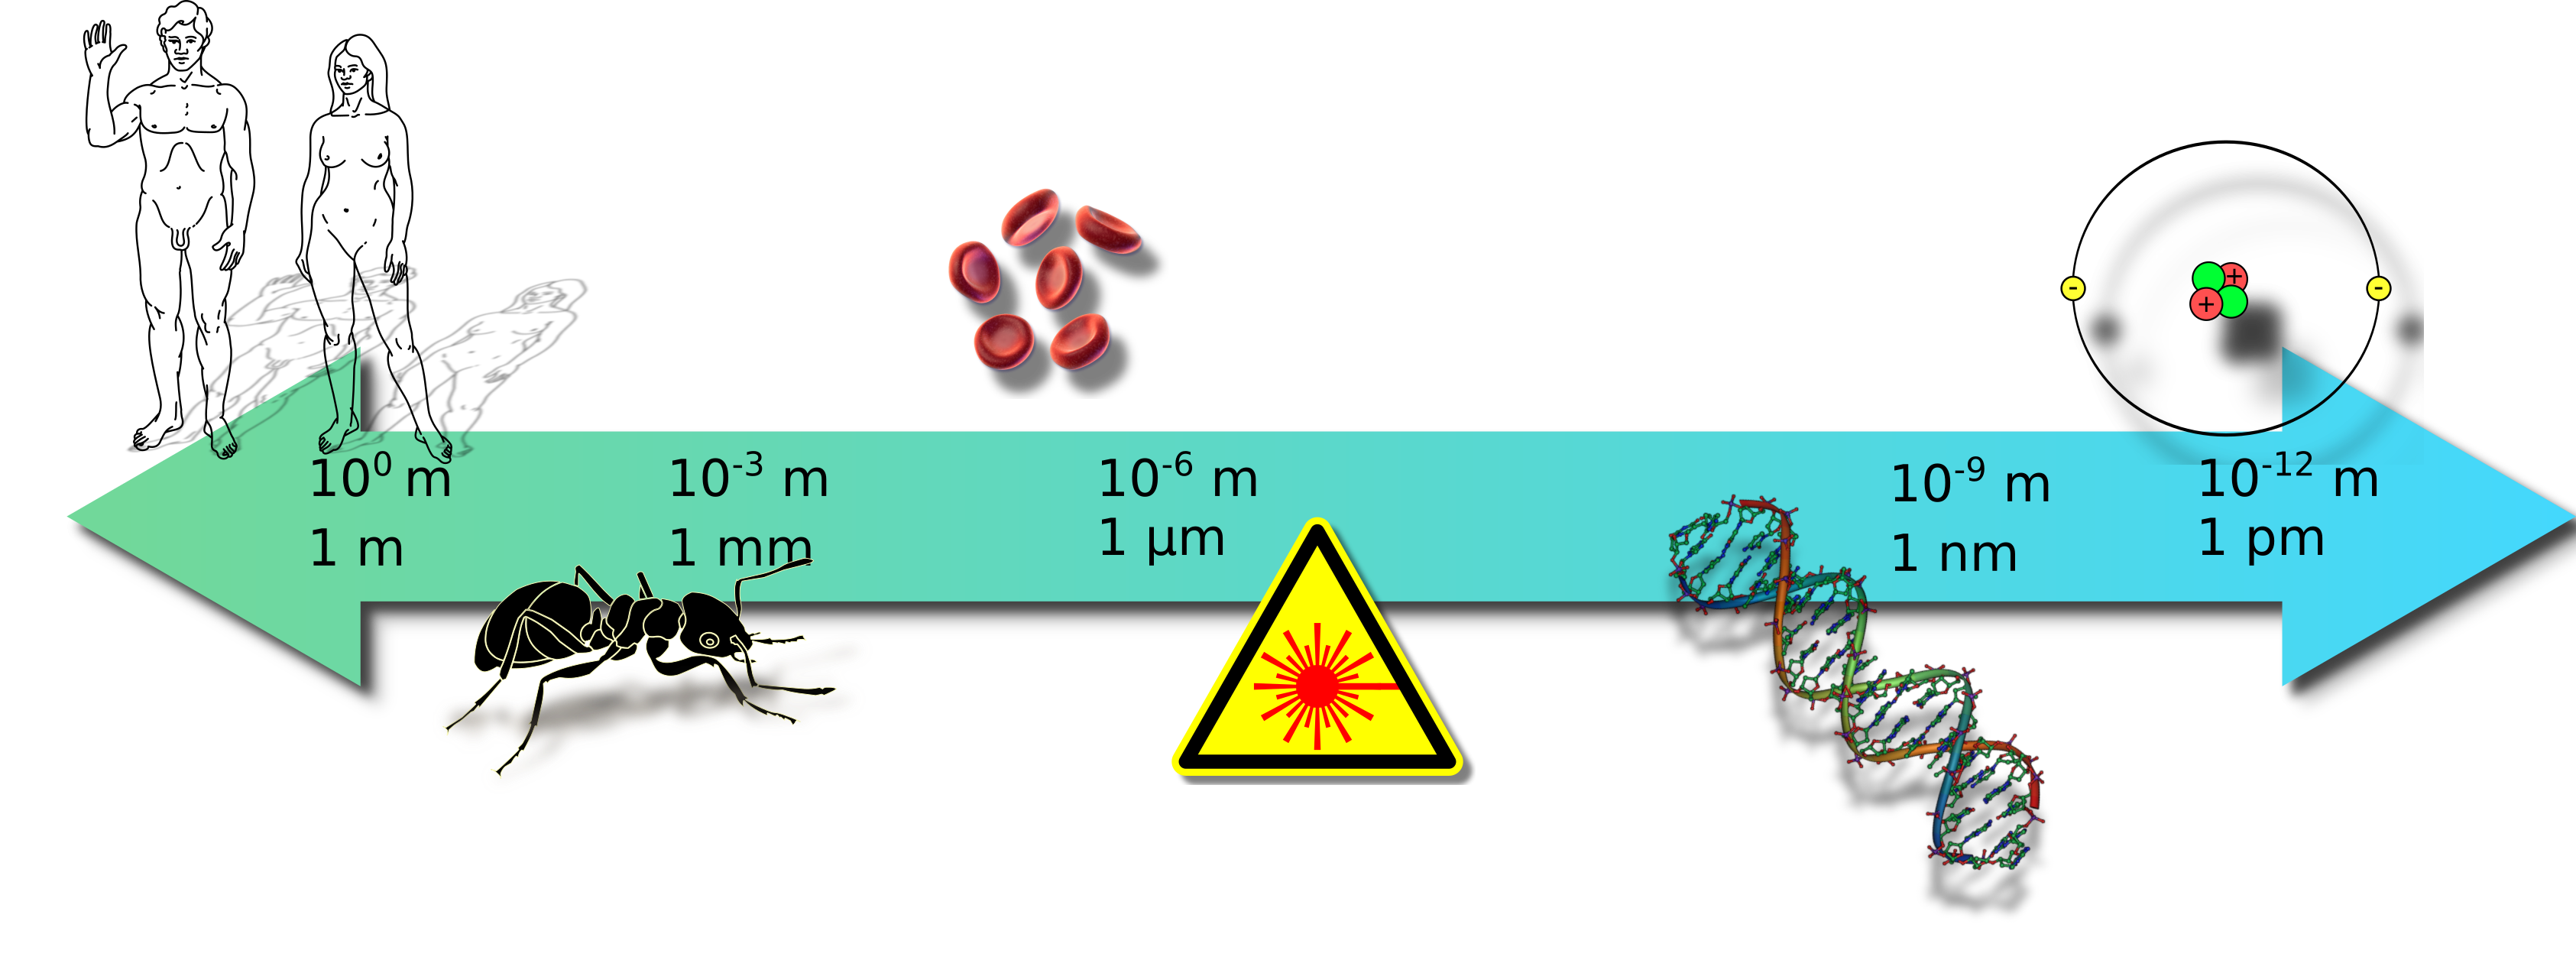
\includegraphics[width=\textwidth]{scale.png}
	}
	\label{fig:scale}
	\caption[asd]{Comparativa de órdenes de magnitud. De izquierda a derecha: Escala humana. Insectos. Glóbulos rojos. Longitud de onda de luz. ADN. Radio de un átomo de helio.}
\end{figure}

La idea de la nanotecnología fue vislumbrada por el físico Richard Feynman y expuesta en su charla \emph{``There is plenty room at the bottom''} \citep{Feynman1960}. Aquí Feynman plantea que no existen barreras físicas que impidan manipular sistemas nanométricos, moléculas, o átomos. La era moderna de la nanotecnología comienza con el desarrollo del microscopio de efecto túnel por Binning y Rohrer en 1981 \citep{Binnig1982}, que les hizo ganar el Premio Nobel de Física en 1986. Un microscopio de efecto túnel (STM por sus siglas en inglés \emph{Scanning Tunneling Microscope}), puede superar resoluciones de 0,1 nm de resolución lateral, y 0,01 nm en profundidad, y trabajar en variadas condiciones, sin necesidad de alto vacío o bajas temperaturas. Además de poder resolver átomos, el STM también puede manipularlos \citep{Chen2008}.



\section*{La física de sistemas nanométricos}
El mundo nanométrico es parte de nuestro mundo pero a diferencia del mundo macroscópico al que estamos acostumbrados, son las leyes de la mecánica cuántica las que toman el control. Esto surge de la naturaleza corpuscular de la materia y la cuantización de la energía, que si bien nos olvidamos de ella en el mundo macroscópico, a escala nanométrica toma real importancia, 
